\newpage
\section{Ergebnisse}
Dieses Kapitel stellt die zentralen Ergebnisse des Projekts vor. 
Zunächst wird der entwickelte \acs{aas}-Demonstrator der robocell vorgestellt.
Im Anschluss efolgt die Analyse des eingesetzten \acs{ki}-Modells sowie die Präsentation der beiden Anwendungsfälle. 
Abschließend wird eine Bewertung der verwendeten Softwarelösungen und Tools vorgenommen.

\subsection{AAS-Demonstrator für die robocell}
Im Rahmen dieses Projekts wurde für das Abfüll- und Verschließmodul ein digitaler Zwiling auf Basis der \acs{aas} realisiert.
Dafür wurde ein \acs{aas}-Demonstrator entwickelt, der sowohl auf standardisierte Templates der \acs{idta} als auch auf individuell angepasste Submodelle zurückgreift. 
Der Zwilling wurde als Instanz modelliert, obwohl kein reales physisches Asset als Vorlage diente. 
Die Umsetzung erfolgte dennoch so, als handle es sich um eine konkrete Maschine und nicht nur den Maschinentyp.

Die statische Modellierung wurde vollständig mit dem Package Explorer durchgeführt. 
Alle relevanten statischen Informationen wurden manuell eingetragen. 
Als Hauptdatenquellen dienten technische Dokumentationen der robocell, insbesondere die Betriebsanleitung, sowie Informationen aus dem \acs{plm}-System Agile.
Zeitabhängige Daten der Maschine wurden simuliert und flossen in dynamische Submodelle ein.

\subsubsection{Systemarchitektur}
Die Gesamtarchitektur des Demonstrators basiert vollständig auf containerisierten Komponenten, wodurch eine skalierbare und modulare Struktur entsteht. 
Als zentrale Plattform zur Verwaltung und Bereitstellung der \acs{aas} dient Eclipse BaSyx. 
Ursprünglich war der AASX Server Blazor vorgesehen, dieser wurde jedoch frühzeitig durch BaSyx ersetzt, da die Plattform eine deutlich flexiblere und umfassendere Umgebung für digitale Zwillinge bietet.
Alle Komponenten wurden dabei als Docker-Container implementiert.

Für die Bereitstellung dynamischer Daten bildeten der Maschinensimulator und der Datengenerator die Grundlage.
Der Maschinensimulator war bereits vorhanden und konnte direkt in das System eingebunden werden. 
Der Datengenerator hingegen wurde im Rahmen des Projekts als Node.js-Anwendung neu entwickelt. 
Beide Komponenten stellen die Maschinendaten über einen integrierten \acs{opcua} Server bereit und ermöglichen so die Echtzeitkommunikation mit dem digitalen Zwilling. 
Die Datenübertragung erfolgt über die Databridge, welche die Verbindung zwischen den simulierten Datenquellen und den dynamischen Submodellen der \acs{aas} herstellt.

Zur Speicherung und Analyse der Maschinendaten wurde zusätzlich Telegraf eingesetzt, um die Daten in eine InfluxDB zu übertragen. 
Dies ermöglicht nicht nur die Verarbeitung von Echtzeitdaten, sondern auch die Analyse historischer Datenbestände.

Die zugrundeliegende Architektur ist in Abbildung \ref{fig:Systemarchitektur} dargestellt.

\begin{figure}[htbp]
    \centering
        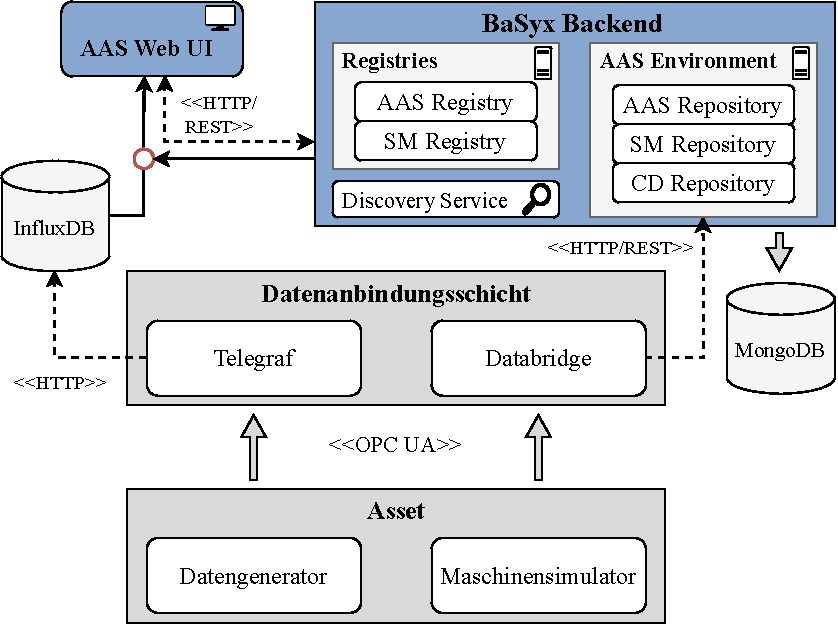
\includegraphics[width=1\textwidth]{Bilder/Ergebnisse/DynamischeDaten/Architektur.pdf}
    \caption{Systemarchitektur AAS-Demonstrator}
    \label{fig:Systemarchitektur}
\end{figure}

Da Einträge in den Discovery Service noch nicht automatisch von stattten gehen wurde zu diesem ein Node.js Skript geschreiben, das diese Funktionalität übernimmt.
Dieses erstellt beim Start der BaSyx-Umgebung automatisch die in einer JSON-Datei hinterlegten Einträge, bei denen das jeweilige Asset mit seiner zugehörogen AAS verknüpft wird.
Dies ist besonders wichtig, um eine AAS finden zu können auch wenn man nur die Asset-ID hat. In dieser Arbeit war dies vor allem zur Abbildung hierarchischer Strukturen sowie für den Anwenungsfall zum DPP notwendig.
Beim Starten der Anwendung werden die Eintröge schließlich automatisch geposted.
In Zukunft erwartet das beu BaSyx das auch automatisch beim Hochladen einer neuen AAS erfolgt und man das nicht mehr selber umsetzen musss, da das sonst sehr aufwendig ist.

Zur Visualisierung der AAS wurde neben der AAS Web UI ebenfalss der Mnestix Browser eingesetzt, da dieser in der Architektur einfach mit dieser ausgetauscht werden kann.
Eine dertailliertere Beschreibung der Tools findet sich in Kapitel !!!.


\subsubsection{Statische Submodelle}

\subsubsection{Dynamische Submodelle}

Für die Inegration des Mashcinenstatus wurde die Databridge eingesetzt.
Für Submodell Kontrollkomponente wurde hierfür ein Submodell entworfen, das den aktuellen Zustand der Maschine abbildet.
Dabei stand ein Plugin zur Verfügung das bereits einen solchen Zustandsautomat abbildet.
Allerdings wurde dieses nicht ausfürlich beschrieben, bzw. nur im Rahmne eines Forschungsprojekts von ... vorgestellt.
Darin wird es beschrieben.
Das von denen entwickelte Vue.js Plugin wurde also angepasst.

Dazu wurde eine Logik implementiert, die wenn das Plugin aktiv ist den Maschinesatuts in regelmäßigen Abständen pollt.
Ändert sich dieser so wird der entsprechende Status gesetzt und zudem die OOperatiuonen die ausgeführt werden können.

Die Kontrollkomponenten ermöglicht also theoretisch die Steuerung der Maschine.
Der Maschinensimulator wurde so konfiguriert das wenn der Status geändert wird zum Beispiel drückt ein Nutzer den Stop Button so wird der Zustand der Maschin, wie im Mashcinesimulator abgebildet gestoppt.
Das ist im Sinne eines richtigen digitalen Zwillings wenn das ganze automatisiert wird könnte zum Beispiel der digitale Zwiloing analig Einfluss auf die Maschine nehmen, zum Beispiel wenn Fehler erkannt werden



Der Macshinensimulator simuliert PackML dabei die Werte über OPC UA
Die Databridge holt die jeweiligen Werte

\subsubsection{Herausforderungen bei der Implementierung}

%KI-Modell
\subsection{Evaluation des KI-Modells}
\subsubsection{Bewertung des prototypischen KI-Einsatzes}
\subsubsection{Ausblick: Predictive Maintenance}
\subsubsection{Weiterführende Einsatzmöglichkeiten}

% Digitaler Produktpass
\newpage
\subsection{Anwendungsfall Digitaler Produktpass}
\subsubsection{Abbildung des PCF}
Zur Abbildung des \acs{pcf} der Gesamtmaschine wurde ein Mechanismus in der AAS Web UI integriert. 
Im Visualisierungsbereich wurde eine Schaltfläche implementiert, über die die Aggregation der CO\textsubscript{2}-Äquivalente ausgelöst werden kann. 
Beim Betätigen dieser wird eine \acs{http}-GET-Anfrage an den Microservice gesendet, der die Berechnung durchführt.

Der Microservice, der ebenfalls als Docker-Container implementiert wurde, reagiert auf die Anfrage und startet den Berechnungsprozess. 
Der Ablauf ist in Abbildung \ref{fig:SequenzdiagrammPCF} als Sequenzdiagramm dargestellt.

\begin{figure}[htbp]
    \centering
        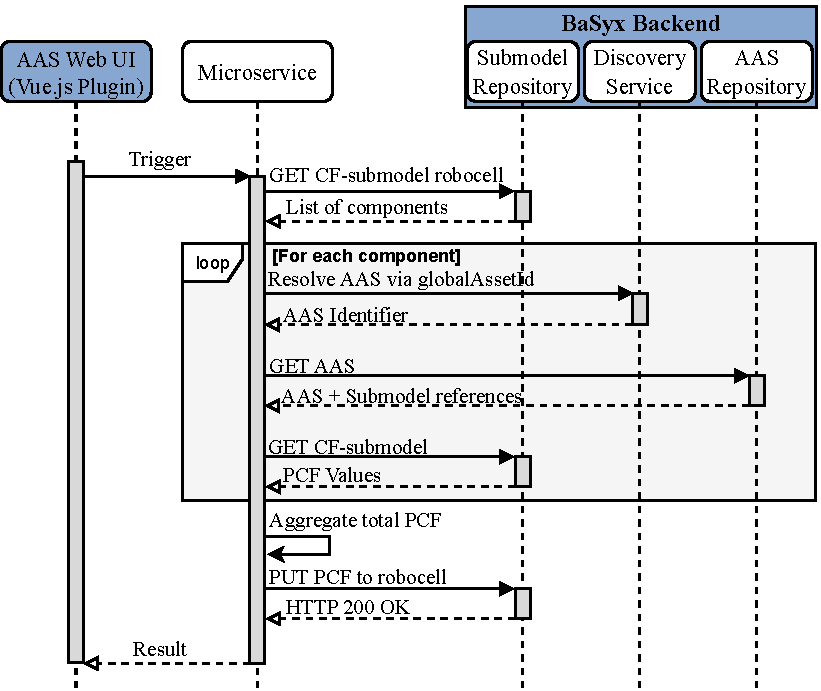
\includegraphics[width=1\textwidth]{Bilder/Ergebnisse/DPP/AggregationNue.pdf}
    \caption{Sequenzdiagramm zur Aggregation des PCF}
    \label{fig:SequenzdiagrammPCF}
\end{figure}

Der Microservice nutzt die \acs{rest}-Schnittstelle des Submodel Repositories der AAS Environment, um zunächst alle in der Komponentenliste des \acs{cf}-Submodells der robocell hinterlegten Komponenten auszulesen. 
Mithilfe des Discovery Service werden auf Basis ihrer globalAssetIds die zugehörigen Komponenten-\acs{aas} identifiziert und anschließend vom AAS Repository abgerufen.
Für jede dieser Komponenten wird geprüft, ob ein \acs{cf}-Submodell vorhanden ist. 
Falls dies zutrifft, wird das Submodell ausgelesen und die enthaltenen \acs{pcf}-Werte extrahiert.

Aus den ermittelten Einzelwerten berechnet der Microservice die aggregierten CO\textsubscript{2}-Äquivalente für die Phasen Produktion, Material sowie Cradle to Gate. 
Die berechneten Werte werden abschließend in das \acs{cf}-Submodell der Haupt-\acs{aas} der robocell geschrieben und stehen dort strukturiert zur Verfügung.

Nach Abschluss der Berechnung sendet der Microservice eine Bestätigung an das Plugin zurück. 
Dieses reagiert darauf, indem es das aktualisierte \acs{cf}-Submodell über die \acs{rest}-Schnittstelle der AAS Environment erneut abfragt. 
Die relevanten Submodellelemente werden dabei herausgefiltert und in der Benutzeroberfläche aktualisiert. 
Dadurch werden die aggregierten \acs{pcf}-Werte unmittelbar sichtbar, ohne dass ein manuelles Neuladen erforderlich ist.

Abbildung \ref{fig:PluginAggregation} zeigt die entsprechende Visualisierung. 
Auf der linken Seite sind die berechneten CO\textsubscript{2}-Äquivalente dargestellt, auf der rechten Seite die zugehörigen Lebenszyklusphasen.

\begin{figure}[htbp]
    \centering
        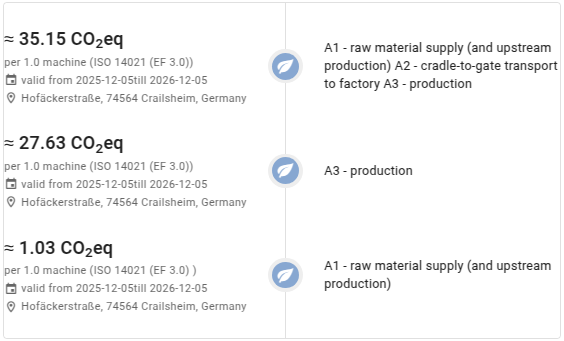
\includegraphics{Bilder/Ergebnisse/DPP/PluginAggregation.png}
    \caption{Visualisierung der aggregierten PCF-Werte im Plugin}
    \label{fig:PluginAggregation}
\end{figure}

Die beschriebene Lösung ermöglicht es, den \acs{pcf} dynamisch auf Basis der in der Komponentenliste referenzierten Steuerungselemente zu berechnen. 
Auch wenn derzeit nur acht Siemens-Komponenten berücksichtigt werden, lässt sich die Liste bei Verfügbarkeit weiterer Komponenten-\acs{aas} unkompliziert erweitern, sodass sukzessive die gesamte Maschine in die Berechnung einbezogen werden kann.

Perspektivisch lässt sich die Berechnung zudem um weitere Lebenszyklusphasen wie Nutzung oder Entsorgung ergänzen, um eine ganzheitliche Betrachtung von der Herstellung bis zum Lebensende eines Produkts bzw. einer Maschine zu ermöglichen.
Darüber hinaus könnte auch der \acs{tcf} berücksichtigt werden, beispielsweise im Rahmen der Auslieferung einer Maschine, wodurch eine noch umfassendere Bilanzierung der Umweltauswirkungen ermöglicht wird.

\subsubsection{Rollenbasierter Zugriff auf Submodelle}
Eine Möglichkeit, die im \acs{dpp} enthaltenen Informationen einzusehen, bietet die AAS Web UI. 
Ist \acs{rbac} aktiviert, wird der Benutzer beim Aufruf der Oberfläche zur Keycloak-Anmeldeseite weitergeleitet. 
Wie in Abbildung dargestellt, kann der Nutzer sich dort mit dem in Keycloak definierten Nutzernamen und Passwort anmelden.

\begin{figure}[htbp]
    \centering
        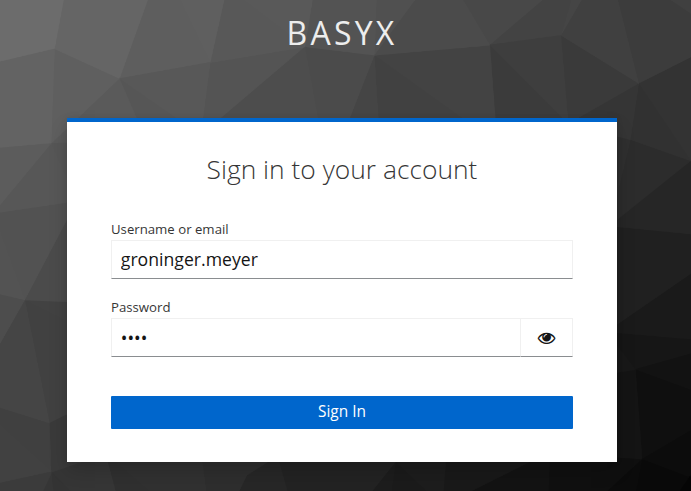
\includegraphics[width=0.7\textwidth]{Bilder/Ergebnisse/DPP/KeycloakAnmeldeSeite.png}
    
    \caption{Keycloak-Anmeldeseite für die AAS Web UI}
    \label{fig:SequenzdiagrammPCF}
\end{figure}

Nach erfolgreicher Authentifizierung erhält der registrierte Client (AAS Web UI) ein Zugriffstoken, das die Rolleninformationen des Nutzers enthält.  
Dieses Token wird im Hintergrund an die angebundenen BaSyx-Komponenten (z.\,B. AAS Environment, Registry) weitergegeben.  
Die Entscheidung über die tatsächliche Zugriffsberechtigung trifft dabei nicht die AAS Web UI, sondern der jeweilige Service, indem er die im Token enthaltenen Rollen gegen die hinterlegten RBAC-Regeln prüft.

+++ Wie ist es wenn nicht alles konfiguriert \\
Beipsiel an Rolle Servgice kann nicht shocladen z.B.\\
 Funkltioniert alles +++\\

Alternativ ist auch ein direkter Zugriff über die \acs{api} möglich, etwa durch technische Clients oder externe Anwendungen.  
In diesem Fall muss das Zugriffstoken aktiv über den Token-Endpunkt des entsprechenden Realms bei Keycloak angefordert und anschließend im \acs{http}-Header der Anfrage übermittelt werden.  
Die Autorisierung erfolgt analog zur Web-Oberfläche durch die jeweiligen BaSyx-Komponenten basierend auf den Rollen im Token und den definierten \acs{rbac}-Konfigurationen.

+++ Mit Postman zeigen +++\\
+++ Für jede Rolle +++\\

+++ Fazit +++ \\

Zeigt dass sich differenzierte Zugriffskontrollen auf Submodell-Ebene technisch realisieren lassen. 
Dies bietet Potenzial für zukünftige Szenarien, bei denen sensible Nachhaltigkeitsdaten nur bestimmten Akteuren entlang der Wertschöpfungskette zugänglich gemacht werden sollen.

\subsection{Anwendungsfall automatisierte Generierung der AAS}
% \subsection{Einsatzmöglichkeiten von KI im Kontext der Verwaltungsschale}
% \subsubsection{Generierung von Verwaltungsschalen}
% \subsubsection{Anomaliererkennung}
% \subsubsection{Weiterführende Einsatzmöglichkeiten}

%Evaluation der eingesetzten Software
\subsection{Evaluierung eingesetzter Tools und Software}
\subsubsection{AASX Package Explorer}
\subsubsection{Eclipse AASX Server}
\subsubsection{BaSyx}
\subsubsection{Mnestix Browser}
Optional davor halt nicht drauf eingeganen\dots